% ********** Scenario **********

\chapter{Scenario}

We propose a simple application to analyze the behaviour of the protocol. The
scenario is of a home monitoring application, which detects gas leaks.
The Sparrowv3 nodes have been equipped with methane sensors and the house has
an alarm system. If methane levels increase past a threshold value, the alarm
must be raised.

\begin{figure}[ht]
	\begin{center}
		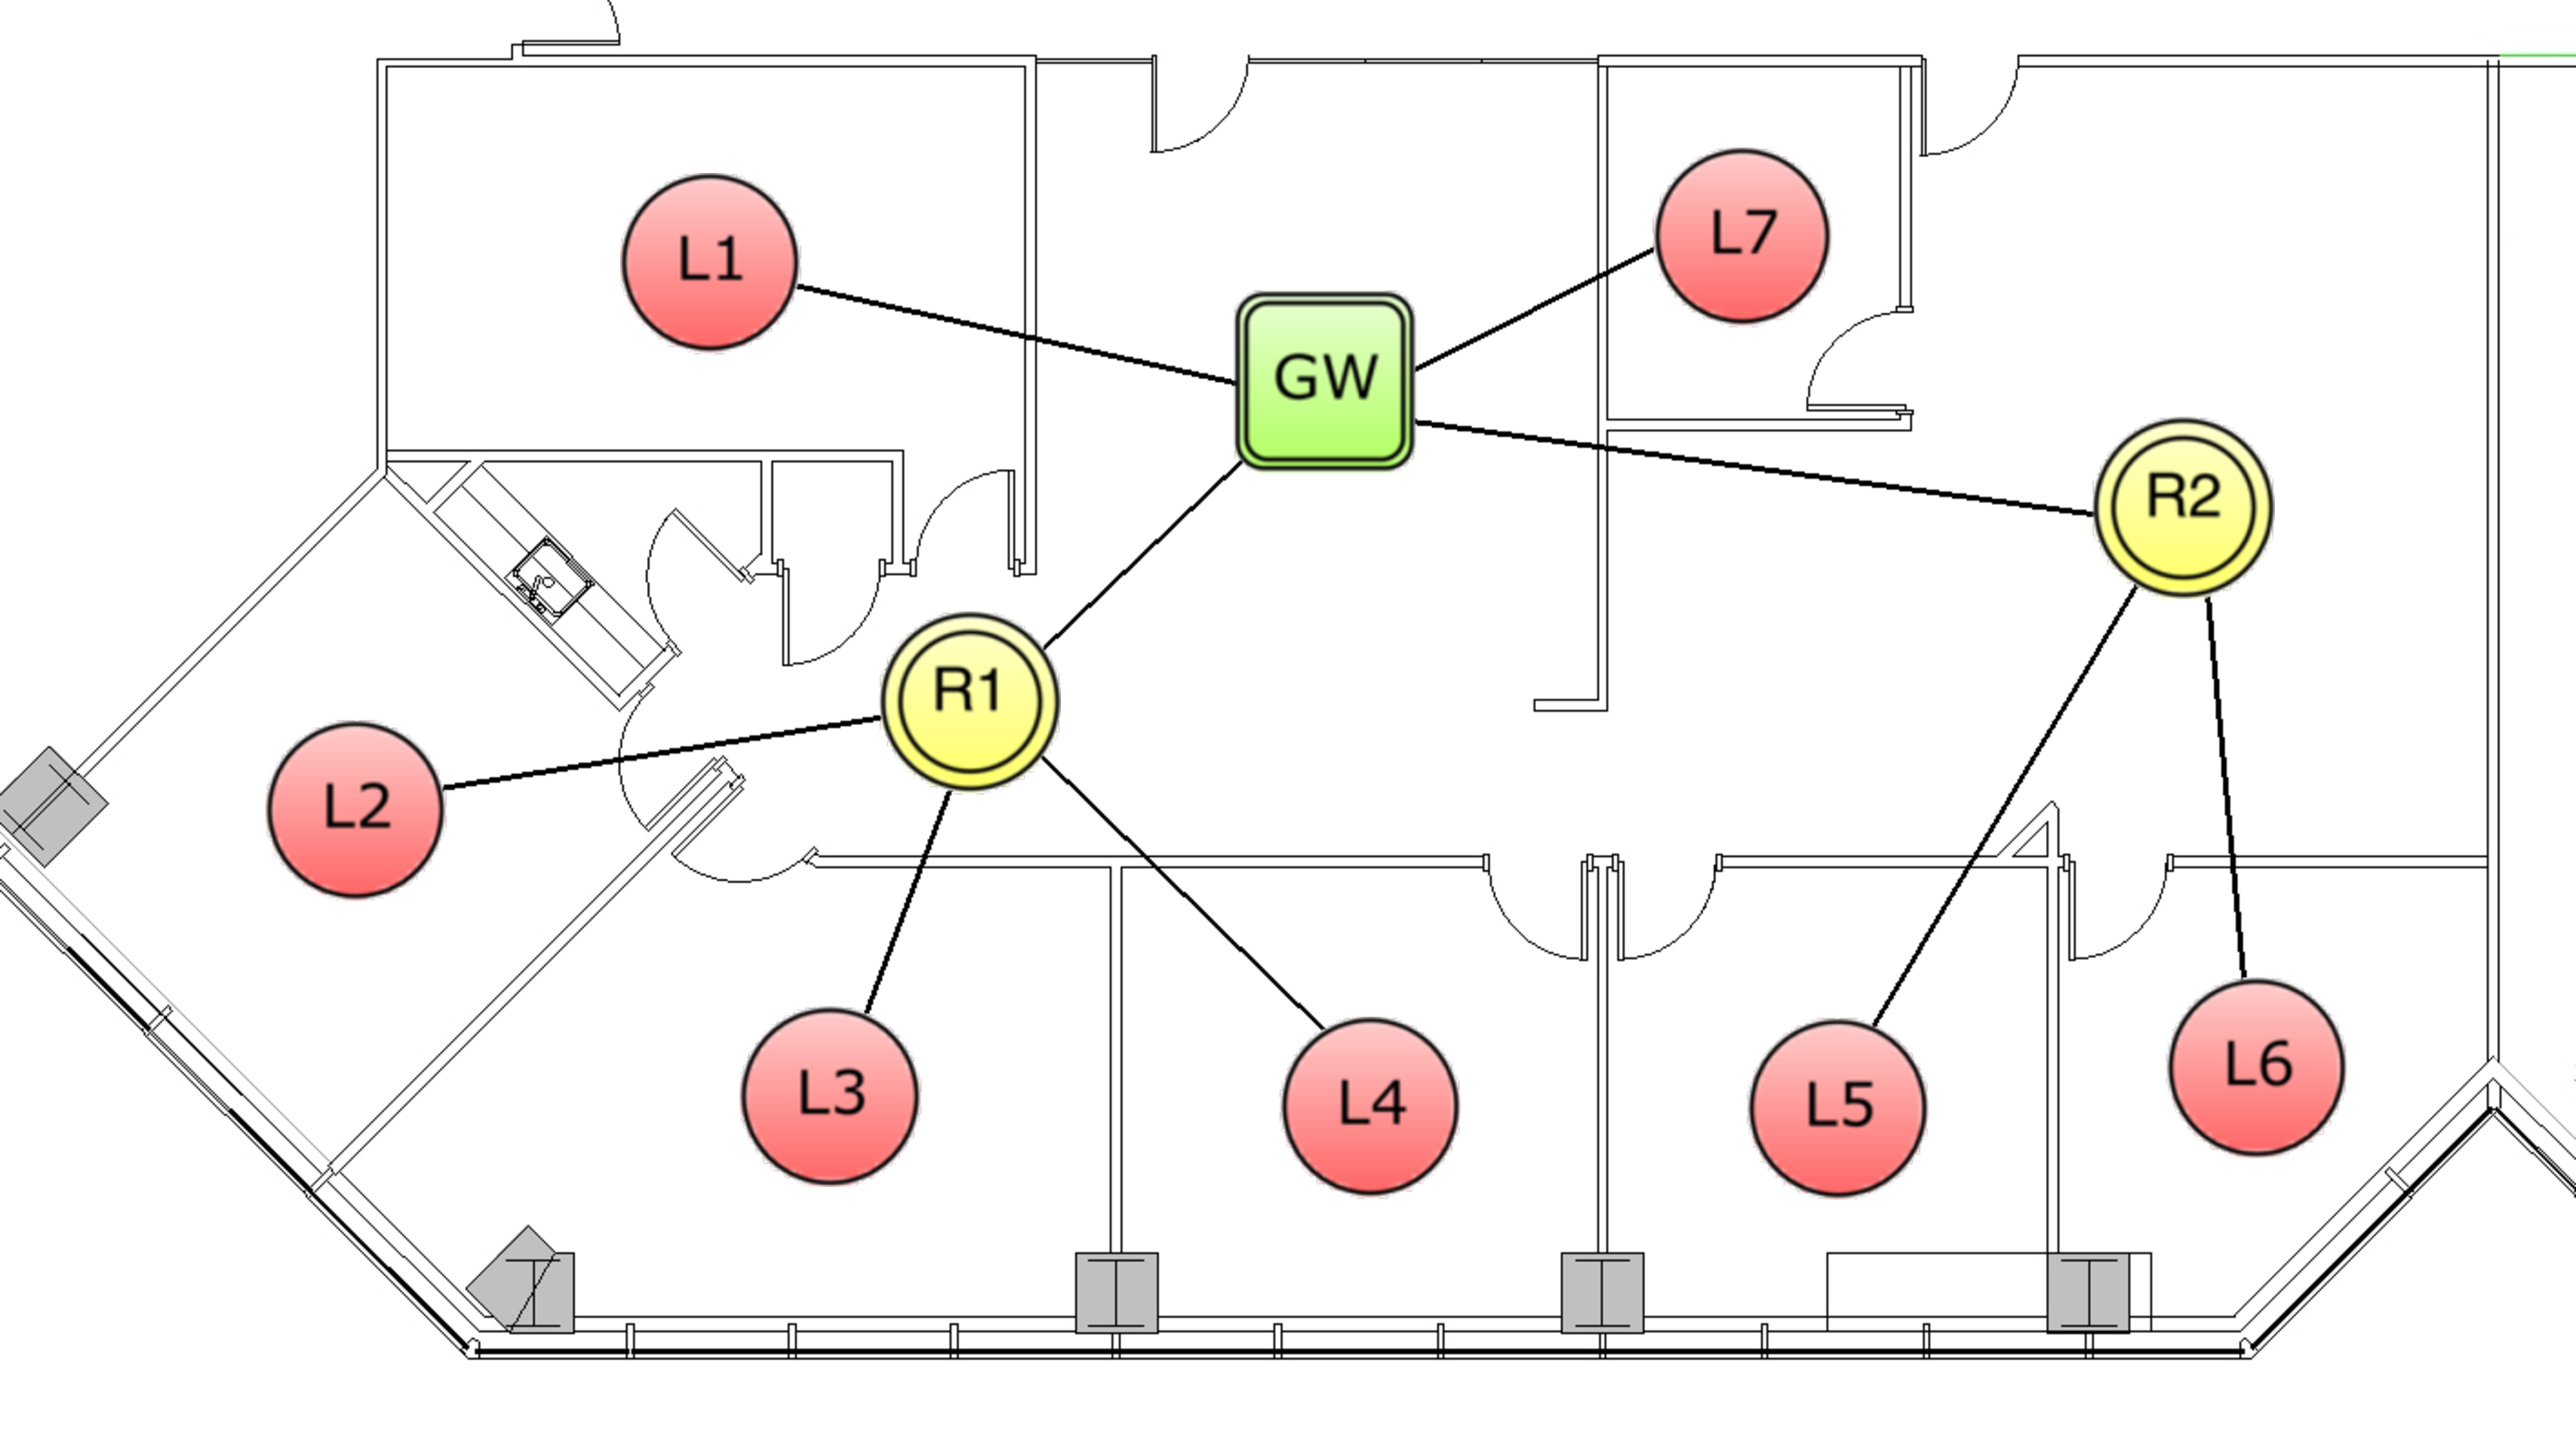
\includegraphics[width=\textwidth]{img/scenario.pdf}
	\end{center}
	\caption{\small \itshape{Sparrow home deployment
	scenario\protect\footnotemark}}
\end{figure}
\footnotetext{Image taken from
\url{http://edgchicago.files.wordpress.com/}}

The network gateway is connected to the alarm controller, root nodes are placed
in intersection points throughout the house and leaf nodes are placed so as to
cover the entire environment. After power on the gateway starts transmitting
Router Advertisements. Next the root nodes are brought online. Both are in
range of the gateway so they can register to it. Leaf nodes are brought online.
Leaf nodes L1, L4 and L7 are in range of the root node, however, L4 is far from
it and the gateway's signal strength is poor, whereas R1's signal strength is
good, so only L1 and L7 register to the gateway and L4 registers to R1. L2, L3,
L5 and L6 are in range of R1 and, respectively, R2. L2 and L3 register to R1
and L5 and L6 register to R2.

In case of a gas leak the alarm must be raised in as short a time as possible.
If a node's measurement rises above a threshold level it sets a flag in the
next packet to be transmitted. Its parent node will forward this packet towards
the gateway. When the packet arrives at the gateway, the data is analysed and,
if the flag is found, the alarm is raised.

% ********** End of Scenario **********
